\def\year{2022}\relax
\documentclass[letterpaper]{article}
% DO NOT CHANGE THIS
\usepackage{aaai22} % DO NOT CHANGE THIS
\usepackage{times} % DO NOT CHANGE THIS
\usepackage{helvet} % DO NOT CHANGE THIS
\usepackage{courier} % DO NOT CHANGE THIS
\usepackage[hyphens]{url} % DO NOT CHANGE THIS
\usepackage{graphicx} % DO NOT CHANGE THIS
\urlstyle{rm} % DO NOT CHANGE THIS
\def\UrlFont{\rm} % DO NOT CHANGE THIS
\usepackage{graphicx} % DO NOT CHANGE THIS
\usepackage{natbib} % DO NOT CHANGE THIS
\usepackage{caption} % DO NOT CHANGE THIS
\DeclareCaptionStyle{ruled}%
{labelfont=normalfont,labelsep=colon,strut=off}
\frenchspacing % DO NOT CHANGE THIS
\setlength{\pdfpagewidth}{8.5in} % DO NOT CHANGE THIS
\setlength{\pdfpageheight}{11in} % DO NOT CHANGE THIS
%
% PDF Info Is REQUIRED.
% For /Title, write your title in Mixed Case.
% Don’t use accents or commands. Retain the parentheses.
% For /Author, add all authors within the parentheses,
% separated by commas. No accents, special characters
% or commands are allowed.
% Keep the /TemplateVersion tag as is
\pdfinfo{
/Title (Explaining Models for Brain Network Classification)
/Author (Keanelek Enns, Tengkai Yu, Alex Thomo, Venkatesh Srinivasan)
/TemplateVersion (2022.1)
}

% Specify path to images
\graphicspath{ {./img/} }

% NOT SURE IF THESE PACKAGES ARE ALLOWED
\usepackage{amsmath}
\usepackage{amsfonts}

\author{
Keanelek Enns, Tengkai Yu, Alex Thomo, Venkatesh Srinivasan\\
}
\affiliations {
University of Victoria 3800 Finnerty Road Victoria, BC V8P 5C2\\
}

\title{Explaining Models for Brain Network Classification}

\begin{document}
\maketitle

\begin{abstract}
TODO
\end{abstract}



\section{Introduction}

%Not sure where this will fit in, but it should be in the intro for referencing the "original paper"
In their paper, "Explainable Classification of Brain Networks via Contrast Subgraphs" (referred to as the original paper from here on),
Lanciano \emph{et al.} define a graph embedding technique using \emph{contrast subgraphs} \cite{lanciano2020}. We define contrast subgraphs later in the paper.

There are a number of different areas we could focus on:
\begin{enumerate}
    \item Autism Spectrum Disorder and its impact
    \item Model Explainability and Interpretability (explainable models vs explanation techniques for black box models)
\end{enumerate}

Contributions:
\begin{enumerate}
    \item Replication of Lanciano et al \cite{lanciano2020} + replication package
    \item Improvements to Lanciano et al's technique + discriminative edges technique + graph embedding evaluation module
    \item Using black box models on dataset (DNN and GNN)
    \item Investigate explanation techniques for black box models
\end{enumerate}



\section{Related Work}

% Manuscripts page: http://fcon_1000.projects.nitrc.org/indi/abide/manuscripts.html

Talk about the shortcomings of the work from lanciano here \cite{lanciano2020}?

\section{Preliminaries}
% We need to do more research on the dataset and consider using the ABIDE II dataset instead of just ABIDE I. It looks like only ABIDE I has been preprocessed from the link below, but perhaps someone has preprocessed ABIDE II in a similar fashion.

% http://preprocessed-connectomes-project.org/abide/index.html

% https://www.frontiersin.org/10.3389/conf.fninf.2013.09.00041/event_abstract
\textbf{Data.}
A common group of data sets were used for the experiments of this paper.
Data from the Autism Brain Imaging Data Exchange (ABIDE) project \cite{craddock2013} was processed by Lanciano \emph{et al.}. % I'm not actually sure if it was processed by them, their wording is strange.
This processing resulted in groups of simple, undirected, and unweighted graphs (brain networks) defined over a common set of 116 vertices.
The vertices of the brain networks correspond to regions of interest (ROIs) in the brain, thus we are studying a special case of graph classification where all considered graphs possess the same set of vertices (i.e. regions of the brain which are, naturally, common to all brains).
This concept is called \emph{node identity awareness}.

The edges of each brain network correspond to functional (as opposed to structural) connections in the brain.
For a more thorough discussion of the data sets used and the processing that was performed by Lanciano \emph{et al.}, please see section 5 of the original paper \cite{lanciano2020}.

\textbf{Notation.}
We reuse the notation specified in the original paper and reiterate the important notation here.

Let the $i^{th}$ brain network be represented as an undirected, unweighted graph $G_i = (V, E_i)$, where $V$ is the common vertex set representing the 116 ROIs of the brain as discussed previously (i.e. $|V| = 116$) and $E_i$ is the set of edges belonging to $G_i$ (note: $E_i \subset V \times V$).

Let a \emph{summary graph} corresponding to a set of brain networks $\mathcal{A}$ be a weighted, undirected graph $G^{\mathcal{A}} = (V, w^{\mathcal{A}})$, where $w^{\mathcal{A}}: V \times V \rightarrow \mathbb{R}_+$ is a weight function that assigns a value to each pair of vertices in $V$.
For vertices $u,v \in V$, we define $w^{\mathcal{A}}(u,v)$ to be the fraction of networks in $\mathcal{A}$ that contain the edge $(u,v)$.

\section{Contrast Subgraphs} \label{cs}

A contrast subgraph is defined as a subset of vertices that induces a dense subgraph in one graph and a sparse subgraph in another, assuming that the graphs share a common vertex set.
We echo the problem definition of finding contrast subgraphs from the original paper.

\emph{Problem 1 (Contrast Subgraph). Given two sets of observation graphs, i.e. the condition group $\mathcal{A} = \{G^{\mathcal{A}}_1, . . . , G^{\mathcal{A}}_{|\mathcal{A}|}\}$ and the control group $\mathcal{B} = \{G^{\mathcal{B}}_1, . . . , G^{\mathcal{B}}_{|\mathcal{B}|}\}$, and corresponding summary graphs $G^{\mathcal{A}} = (V, w^{\mathcal{A}})$ and $G^{\mathcal{B}} = (V, w^{\mathcal{B}})$, we seek to find a subset of vertices $S^* \subseteq V$ that maximizes the contrast subgraph objective}
\begin{align*}
    \delta (S) = \sum_{u,v \in S} \left(w^{\mathcal{A}}(u,v) - w^{\mathcal{B}}(u,v) - \alpha\right)
\end{align*}
\emph{where $\alpha \in \mathbb{R}_+$ is a user-defined parameter.}

The original paper also defines a symmetric variant of the contrast subgraph problem (\emph{Problem 2}) which shares the same definition of \emph{Problem 1}, but with an alternative objective

\begin{align*}
    \sigma (S) = \sum_{u,v \in S} \left(|w^{\mathcal{A}}(u,v) - w^{\mathcal{B}}(u,v)| - \alpha\right)
\end{align*}

The parameter $\alpha$ is used to penalize large contrast subgraphs.
It can be adjusted to vary the proportion of edges that are considered detrimental to the contrast subgraph objective.

These problems can be simplified to finding a set of vertices that induce a dense subgraph in the difference of the two summary graphs.
Consider the difference network  $G^{\mathcal{A} - \mathcal{B}} = (V, w^{\mathcal{A} - \mathcal{B}})$, where \\ $w^{\mathcal{A} - \mathcal{B}}(u,v) = w^{\mathcal{A}}(u,v) - w^{\mathcal{B}}(u,v), \forall u,v \in V$.
In this context, finding a contrast subgraph is equivalent to finding a dense subgraph in the difference network (a dense subgraph is one that maximizes the appropriate objective function).
% What I was trying to say with the parenthesis is that we are defining density in that way, since there are multiple definitions. We should probably be more clear though, as I didn't fully understand after revisiting what I had written some time ago.

Note that contrast subgraphs themselves do not constitute a graph embedding technique, but they can be used in the following ways to embed a graph.

\textbf{Problem 1.}
The original authors use contrast sugbraph overlap to create two features for each brain network.
Because the problem is asymmetric, two contrast subgraphs are obtained.
One is found using the difference network $G^{TD - ASD}$ (which is the result of subtracting the summary graph $G^{TD}$ from the summary graph $G^{ASD}$) and the other is found using $G^{ASD - TD}$.
Each feature corresponds to the number of edges in common between the brain network and each contrast subgraph.
reference figure representing problem 1\ref{fig:prob1} 

\begin{figure}
    \centering
    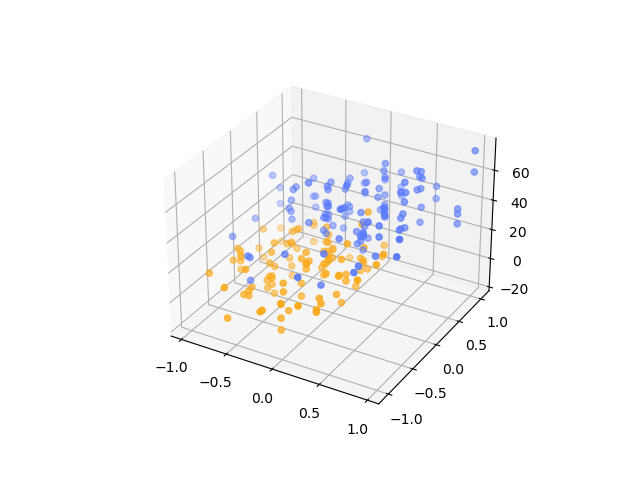
\includegraphics[width=\columnwidth, keepaspectratio=true]{test.png}
    \caption{Show a representative plot for problem 1}
    \label{fig:prob1}
\end{figure}

\textbf{Problem 2.}
Only one contrast subgraph is obtained for this embedding technique.
The contrast subgraph is used to induce subgraphs in both of the summary graphs (i.e. $G^{TD}$ and $G^{ASD}$) as well as each individual brain network.
The distances, computed as the $L_1$ norms, from the induced brain network to each summary graph are then used as the two features for this embedding.
reference figure representing problem 2 \ref{fig:prob2}

\begin{figure}
    \centering
    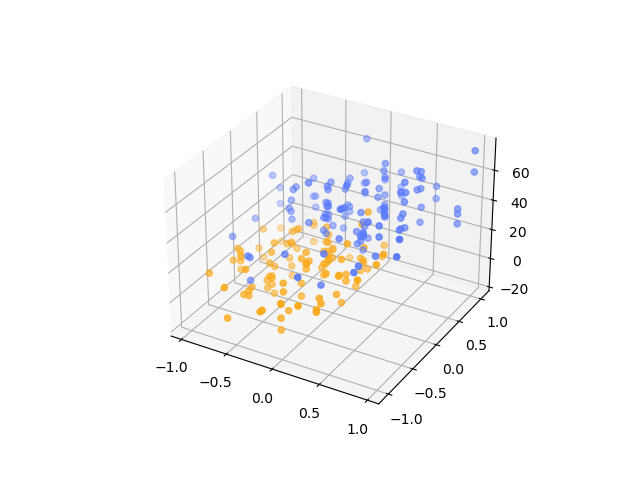
\includegraphics[width=\columnwidth, keepaspectratio=true]{test.png}
    \caption{Show a representative plot for problem 2}
    \label{fig:prob2}
\end{figure}




\section{Improvements} \label{improvements}

Even after optimizations, the original contrast subgraph embedding technique used is quite slow, and the accuracy is not far above the baseline accuracy (we define this as the accuracy obtained when the most dominant class is always predicted).
Therefore we turned our attention to developing improvements for the contrast subgraph embedding technique.

\textbf{Quadratic Programming.}
We looked further into the work by Cadena \emph{et al.} which was repurposed by the original authors.
When creating a mathematical problem formulation for finding a dense subgraph in a signed network, Cadena \emph{et al.} propose a quadratic programming problem.
In their study, they choose to approximate the quadratic program with a semidefinite program and a rounding technique \cite{cadena2016}.
Lanciano \emph{et al.} then use this implementation to find a contrast subgraph in their context.

However, because this study aims to find a dense subgraph in a small difference network (116 by 116), it seemed reasonable to implement a QP solver to solve the problem directly.
We used a Python library named CVXOPT\footnote{This library can be found at \url{https://cvxopt.org/}}.
None of the QP solver libraries we found were able to restrict potential solution vectors to discrete values such as \{-1,1\} (i.e. out or in), so we restricted solution values to [-1,1] rounding positive values to 1 and non-positive values to -1.

The speed increase that resulted from changing the solver was significant as we will discuss in section \ref{results}.

\textbf{Local Search Optimization.}
The QP and SDP solvers only approximate the densest subgraph, so a local search step is used to improve the density of the chosen subgraph.
The localSearch algorithm developed by Tsourakakis \emph{et al.} \cite{tsourakakis2013} and used by both Cadena \emph{et al.} and the original authors works by considering the density of the subgraph if each vertex outside the subgraph were to be added to the subgraph, adding them when it increases the density.
This is repeated until all the vertices have been considered.
Afterwards, the algorithm seeks to remove a single vertex from the subgraph and does so if it finds one that increases the density.
This process is then repeated until a maximum number of iterations have been reached, or no vertices can be added or taken away from the subgraph to increase its density.
The pseudocode for the original algorithm can be found in the paper by Tsourakakis \emph{et al.} \cite{tsourakakis2013}.

Considering the goal of the local search algorithm is to increase the density of the subgraph, we made a modification to the algorithm such that it attempts to remove as many vertices as it can in each iteration (removing them only if they increase the density).
This modified local search algorithm can be seen in algorithm 1, and was found to increase the accuracy of the classifiers that used it over the original implementation.

\textbf{Top-k Contrast Subgraphs.}
Finally, we follow the original authors' suggestion for future work and use the top-k contrast subgraphs.
For the sake of time, we did not implement it according to Balalau \emph{et al.} \cite{balalau2015} as suggested, but instead we took the approach described by Tsourakakis \emph{et al.} in section 4.1 of their paper \cite{tsourakakis2013} and simply removed the vertices of each contrast subgraph that was found and searched for a new contrast subgraph among the remaining vertices of the graph.

The resulting k vectors (or points) for each new brain network were added together to obtain the final embedding.



\section{Discriminative Edges}
In section 5.1 of the original paper, it was shown that the degrees of each vertex in the studied brain networks did not vary significantly between the two classes \cite{lanciano2020}, yet the contrast subgraphs are defined as a set of vertices, and every edge induced by these vertices is used for classification.
In light of this, we thought it would be beneficial to consider only the \emph{edges} that are important for distinguishing between the classes.

The discriminative edges (DE) embedding technique employs a very simple computation for calculating the similarity of a new brain network with each of the summary graphs for ASD and TD brain networks.
Initially, the idea was to identify the $n$ most positive edges and the $n$ most negative edges in the difference network $G^{ASD - TD}$.
These are the edges with the greatest disparity between the two classes (positive edges are more common in ASD brain networks, and negative edges are more common in TD brain networks), and are thus, the most discriminative edges.
For each new brain network $G_i$, we calculate the dot product of the n most positive edges in $G^{ASD - TD}$ with the corresponding edges of $G_i$ (in this case, $G_i$ is unweighted, so present edges have a value of 1, and edges that are not present have a value of 0, however, this calculation would still be effective if $G_i$ were weighted).
This gives $G_i$'s similarity with the ASD class.
A similar calculation is done for the negative edges to give the similarity with the TD class.
These similarities are used as the two features of the technique.

With this incredibly simple algorithm, we achieved results that were very similar to those obtained from the contrast subgraph technique.
However, with further improvements, DE managed to surpass the performance of the contrast subgraph technique whilst remaining computationally efficient.

Rather than ignoring the values of edges in the difference network corresponding to edges that do not exist in $G_i$, we made use of this information by scaling the edge values of $G_i$ such that nonexistent edges have a value of -1 and present edges continue to have a value of 1 (this scaling can also be applied in the case where $G_i$ is weighted).
This means that not having an edge among the most discriminative edges actually counts against the similarity score for each case.

Finally, we added a third feature to the embedding technique.
This feature is derived in a very similar way, but uses every edge in the calculation, and thereby captures more information.
It is calculated by scaling the edge values of $G_i$ as discussed previously, multiplying each edge to its corresponding edge in the difference network, and summing the values.
This gives one score, a positive value implies similarity with the ASD class, whereas a negative value implies similarity with the TD class.
% Note that we may need to change the order I mentioned here depending on what the figures show in terms of positive and negative scores \ref{fig:DE}



\section{Experiments}



\section{Discussion}
\textbf{Discussion of Node-Identity Awareness and its importance with respect to how we treat the data. We do not need to treat it strictly like a graph as lanciano et al do.}


\section{Conclusion}


\subsection{Future Work}
\begin{itemize}
    \item Consider spaciality of ROIs.
    \item Consider different preprocessing of ABIDE dataset.
    \item Run experiments with ABIDE II (if we don't get to it)
\end{itemize}



\appendix

% References and End of Paper
% These lines must be placed at the end of your paper
\bibliography{refs}
\end{document}
